\documentclass{optica-article}

\journal{opticajournal} % for journals or Optica Open

\articletype{Research Article}

%%%%%%%%%%%%%%%%%%%%%%%%%%  PACKAGES  %%%%%%%%%%%%%%%%%%%%%%%%%%

\usepackage{lineno}
\usepackage{verbatim}
\linenumbers % Turn off line numbering for Optica Open preprint submissions.

\usepackage{graphicx}
\usepackage{subcaption}
\usepackage{float}
\usepackage{amsmath}
\usepackage{bm}
\usepackage{makecell}
\usepackage{xcolor}

\usepackage{ulem}

\begin{document}

\title{Machine learning based retrieval of total ozone column amount and cloud optical depth from irradiance measurements}

\author{Milos Sztipanov,\authormark{1,*} Levente Krizs\'an,\authormark{1} 
Wei Li,\authormark{1} and Knut Stamnes,\authormark{1} }

\address{\authormark{1}Department of Physics, Stevens Institute of Technology, Hoboken, New Jersey, USA\\}

\email{\authormark{*}milostipanov@gmail.com} %% email address is required; see note below about the corresponding author designation

% use {asbstract*} to suppress the copyright line. Copyright information will be added in production

\begin{abstract*} 
A machine learning algorithm combined with measurements obtained by the Norwegian Institute for Air Research (NILU-UV) irradiance meter enable the determination of total ozone column (TOC) amount, radiation modification factor (RMF), and cloud optical depth (COD). 
Operating in the New York City area, a NILU-UV instrument on the rooftop of Stevens Institute of Technology (40.74$^\circ$N, -74.03$^\circ$E) has been used to collect data for several years. 
Inspired by a previous study [Opt. Express \textbf{22}, 19595 (2014)], this research presents an updated neural network-based method for TOC and COD retrieval.
The method presented in this paper provides reliable performance under heavy cloud conditions, and a convenient algorithm for simultaneous retrieval of TOC and COD.
The TOC amounts are presented for 2014-2023, and compared with the look-up table method (LUT) and those obtained from the Ozone Monitoring Instrument (OMI, deployed on NASA's AURA satellite), and COD results for 2014-2019.


\end{abstract*}

%%%%%%%%%%%%%%%%%%%%%%%%%%  body  %%%%%%%%%%%%%%%%%%%%%%%%%%
\section{Introduction}
\label{sec-intro}
Atmospheric ozone plays a crucial role in absorbing ultraviolet UV radiation, thus providing protection to the biosphere, which encompasses all living organisms including ecosystems and humans.
While a moderate amount of UV radiation can stimulate vitamin D production in the skin, excessive exposure to UV radiation poses risks to both humans and most organisms. 
The UV spectral range is known to have harmful biological effects on living organisms and biomolecules. 
Thus, monitoring the total ozone column (TOC) is important. 

Because the importance of monitoring the ozone layer, there is a constant motivation to improve and develop satellite and ground-based ozone amount retrieval techniques. 
In the near past machine learning had shown a great improvement and neural networks have been in the focus of different fields of natural sciences. 
Neural networks showed great flexibility and potential to be adopted to address different problems in cognitive science, information science, computer science, marketing, artificial intelligence, biology, chemistry and other sciences.

Radiative transfer simulations, Machine learning, and computer hardware have developed since 2013, from when we have the latest TOC and COD data from this area, derived by a radial basis function neural network \cite{Fan:2014}.
The two main motivators of this study are 
(i) to follow up on the state and trends of the varying ozone layer in the New York City area and 
(ii) to create an updated machine learning based retrieval technique that is accurate and easy to use.

For radiative transfer modeling AccuRT has been used. 
The main instruments used in this research are the NILU-UV (No.115), which  has been deployed and operated in the New York City area (40.74$^\circ$N, -74.03$^\circ$E) for several years and the Ozone Monitoring Instrument (OMI).

A detailed description of the radiative transfer simulations, retrieval methodology, machine learning and training methods used in this research is provided in the following Sections.
Furthermore, comparisons of results obtained by the neural network and LUT method applied to the NILU-UV data and the OMI results as well as the relationship between the radiation modification factor (RMF) and COD are presented.


\section{Methodology}
\label{sec-method}

The combination of radiative transfer simulations, machine learning methods and irradiance measurements were used to infer TOC and COD. 
The first step was using radiative transfer simulations to create training data for the neural network. 
After the set up of the neural network, the synthetic dataset with the absolute response function (of the NILU-UV) applied to it, was used for training. 
Once the training was done the validation of the results took place. 
This step was followed by preparing the collected NILU-UV raw data to be used as input to the neural network to infer the TOC and COD. Once the TOC results were obtained, they were compared to the OMI values, and statistics were calculated to quantify their similarities/discrepancies.
In the following sections we describe (i) the instrumentation, (ii) the radiative transfer simulations, (iii) the neural network approach, (iv) the NILU-UV and OMI data preparation, (v) the results of our research, and finally (vi) a conclusion.c	


\section{Instrumentation}
\label{sec-instruments}

\subsection{NILU-UV}
\label{sec-niluv}

The NILU-UV No.~115 irradiance radiometer used to collect data employed in this research.
The NILU-UV radiometer measures voltages in each of six channels depending on the magnitude of the downward irradiance at the given channel an its bandwidth and response function. 
The channels of the NILU-UV instrument are centered at 302 nm, 312 nm, 320 nm, 340 nm and 380 nm with $\sim 10$ nm at full width at half maximum (FWHM). 
A sixth channel takes measurements in the visible (or so-called photosyntetically active) PAR range, 400--700 nm with a bandwidth of 300 nm at FWHM.
For the five UV channels the range of the absolute response function of the NILU-UV spans wavelengths from 290 nm to 387 nm.
The NILU-UV instruments were optically characterized (spectral and cosine responses) at the optical laboratory of the Norwegian Radiation Protection Authority (NRPA) in 2005 \cite{Aalerud:2006}.
Figure~\ref{fig:absoluteresponse} shows the absolute response functions $R(\lambda)$ for each channel. 

\begin{figure}[H]
	\centering
	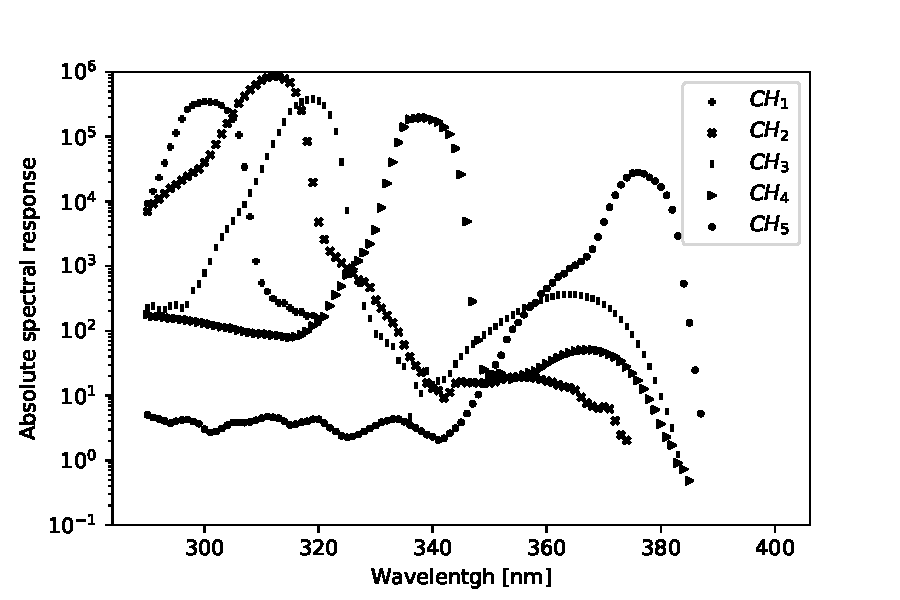
\includegraphics[width=0.7\linewidth]{absolute_response}
	\caption{The absolute spectral response of No. 115 NILU-UV instrument.}
	\label{fig:absoluteresponse}
\end{figure}



The response functions were characterized with a 1 nm resolution.
Throughout this study, channels 1, 3 and 5 were used.
\textcolor{blue}{Channel 3 is significantly less sensitive to ozone abundance than channel 1 so the ratio of the two is an ideal choice for the retrieval. 
At $\lambda = 380 \, \text{nm}$ the ozone cross section is near minimal therefore channel 5 is the least sensitive to ozone but is responsive to clouds, aerosol particles and surface albedo. This makes channel 5 optimal for RMF retrievals.} 
The absolute response of these channels span over the whole range mentioned above dom$[R(\lambda)] = \{\lambda \in \mathbb{Z} \mid 290 \, \text{nm} \leq \lambda \leq 387 \, \text{nm} \}$.



The radiometer has built-in memory to store data and a temperature controller. 
It records data at a 1-minute time resolution. 
Besides the (limited capacity $\sim$ 24 day) built-in memory, data can be recorded and stored by connecting the device to a computer with a RS-232 port. 
The instrument is equipped with moderate bandwidth filters that tend to drift with time; hence the instrument requires a relative calibration (typically once or twice a month). 
The instrument also needs to be absolute calibrated before deployment. 
The total weight of the instrument is 3.3 kg; it is waterproof and designed to operate in harsh environments.

\subsection{OMI}
\label{sec-omi}

The Ozone Monitoring Instrument (OMI) is deployed on NASA’s AURA satellite which is in a Sun-synchronous orbit. 
This satellite was launched on July 15, 2004. 
The OMI is measuring TOC amounts, UV-radiation, and aerosol abundance. 
OMI data are gridded at 0.25 degrees, it has a 780 × 576 (spectral × spatial) pixel CCD detector. 
AURA’s swath is 2600 km and the nadir viewing footprint is 13 km × 24 km.


\section{Radiative transfer simulations}	
\label{sec-simulations}

In order to train the neural network, one needs to provide the training data to the algorithm. 
To create the training (or synthetic dataset), AccuRT was used. 
AccuRT is a unique, state of the art radiative transfer simulation package that was designed to provide a reliable, well-tested, robust, versatile, and easy-to-use radiation transfer tool for coupled (atmosphere and underlying surface) systems {\cite{Knut:2018}}. 
AccuRT uses the discrete ordinate method for the radiative transfer modeling \cite{Knut:1988}.

The desired outputs from the neural network are TOC and COD at 380 nm ($\tau_c{\scriptstyle(380 \, \text{nm})}$).  
The available possible inputs from the NILU-UV are the raw measurements in the 6 channels, and an indirect product of the instrument, the so called radiation modification factor (RMF), that is described as follows:

%REVIEW THIS SECTION ABOUT RMF /put citation from myself? --> this description is from my antarctica paper word to word/
When solar radiation passes through the ozone layer of the atmosphere, a portion of the UVB radiation will be absorbed by ozone, while the portion that penetrates the ozone layer will be multiply scattered or absorbed by air molecules, aerosols, and cloud particles 
\cite{knutbook}. 
To take into account the effects of clouds, aerosol particles, and surface albedo on the UV radiation a radiation modification factor (RMF) is introduced. The RMF is the measured irradiance at wavelength $\lambda$ and solar zenith angle $\theta_0$, $F_m(\lambda,\theta_0,TOC)$, divided by the calculated irradiance, $F_c(\lambda,\theta_0,{ TOC})$, at the same $\lambda$ and $\theta_0$ at the altitude of the site for a cloud- and aerosol-free sky and zero surface albedo.

\begin{equation}
	\label{eq:CLT}
 		RMF =\frac{F_m(\lambda,\theta_0,{ TOC})}{F_c(\lambda,\theta_0,{ TOC})}\times 100.
\end{equation}

In this study the 380 nm channel was used to determine the RMF. 
The RMF defined here is  relatively insensitive to 
the ozone abundance because the ozone absorption cross section is very small at $\lambda=$ 380 nm, whereas the RMF is sensitive to clouds, aerosol particles, and the surface albedo. 
RMF may be larger than 100 when broken clouds are present and the direct beam from the unobscured Sun is measured by the instrument as well as diffuse sky radiation scattered by broken clouds \cite{Dahlback:2003}. 
%Furthermore, snow on the ground enhances the albedo and thus the radiation reflected from the surface. Such a circumstance will increase the downward irradiance and may give RMF values larger than 100 .

The goal was to train the neural network in terms of the measured voltages in each channel at different atmospheric conditions for varying COD ($\tau_c{\scriptstyle(380 \, \text{nm})}$), TOC amounts, and solar zenith angles $\theta_0$. Hence,  the solar spectrum (290 nm - 387 nm) and the resolution of the absolute response functions (1 nm) were used in the AccuRT computations to obtain the irradiances at these wavelengths.

Cloud optical depth can not be used as a direct input to AccuRT. 
The cloud volume fraction ($f_{V,c}$) is used in conjunction with the cloud extinction coefficient to generate the cloud optical depth at 380 nm, $\tau_c{\scriptstyle(380 \, \text{nm})}$. 

The input parameters and their ranges are shown in Table~\ref{tab:accurtinput_ozone}.
20,000 simulations were prepared to be computed.
\textcolor{blue}{For each case a value was randomly selected for $\theta_0$, O$_3$, and $f_{V,c}$} from the presented ranges in Table~\ref{tab:accurtinput_ozone}. 
A Matlab script was used to \textcolor{blue}{cycle through the 20000 prearranged cases and run the individual AccuRT simulations.}

\begin{table}[H]	
	\centering
	\begin{tabular}{|c|c|c|c|}
		\hline
		\textbf{Parameter}	& $\theta_0$ & O$_3$ & $f_{V,c}$  \\
		\Xhline{2\arrayrulewidth}
		\textbf{Minimum	}& 17$^{\circ}$ & 220 DU & $10^{-11}$  \\
		%\hline
		\textbf{Maximum	}& 70$^{\circ}$ & 440 DU & $10^{-6}$ \\
		\hline
	\end{tabular}
	\caption{Input parameters and their ranges for the AccuRT simulations.}
	\label{tab:accurtinput_ozone}
\end{table}

For the simulations the US Standard Atmosphere \cite{USstandardatmosphere} model was used and the surface albedo was chosen to be 0.14 which is typical for cities \cite{Sugawara:2014}.
With the cloud model used (see Sec.~\ref{sec-cloud}), the limits of $f_{V,c}$ are equivalent to min$\{\tau_c(380 \, \text{nm})\} = 0.001526$ and max$\{\tau_c(380 \, \text{nm}) = 152.596$ in terms of COD.
In Table~\ref{tab:accurtinput_ozone} min$\{\theta_0\}$ reflects the lowest possible solar zenith angle at the measurement site, and  max$\{\theta_0\}$ the upper limit to minimize measurement error. 
The minimum of  $\theta_0$ was chosen to be the lowest solar zenith angle throughout the year and the maximum limit was bound to keep the measurement errors low. 
For $\theta_0 > 70^{\circ}$ the impact of cloudiness, the vertical profile of ozone and temperature, the imperfect cosine response of the instrument, and the absolute calibration error reduce the accuracy of the results \cite{Kazantzidis:2009}.


 \subsection{Cloud model}
 \label{sec-cloud}

Clouds were assumed to consist of a collection of homogeneous water spheres having a single-mode log-normal volume size distribution with a specified volume mode radius $r_v=10$ $\mu$m and width $\sigma = 0.2$. 
%The refractive index for pure  water is based on data taken from the literature.
Clouds were placed in the 13$^{th}$ layer in our model. 
This layer is between 2000 m - 4000 m altitude.
A Mie code was used to compute the inherent optical properties of cloud particles.

To convert the cloud volume fraction $f_{V,c}$ to cloud optical depth further computations were done with AccuRT.
Repeated simulations were done to obtain $\tau_c{\scriptstyle(380 \, nm)}$ at different cloud volume fractions.
The result is shown in Figure \ref{fig:codvsvolf} below.

\begin{figure}[H]
	\centering
	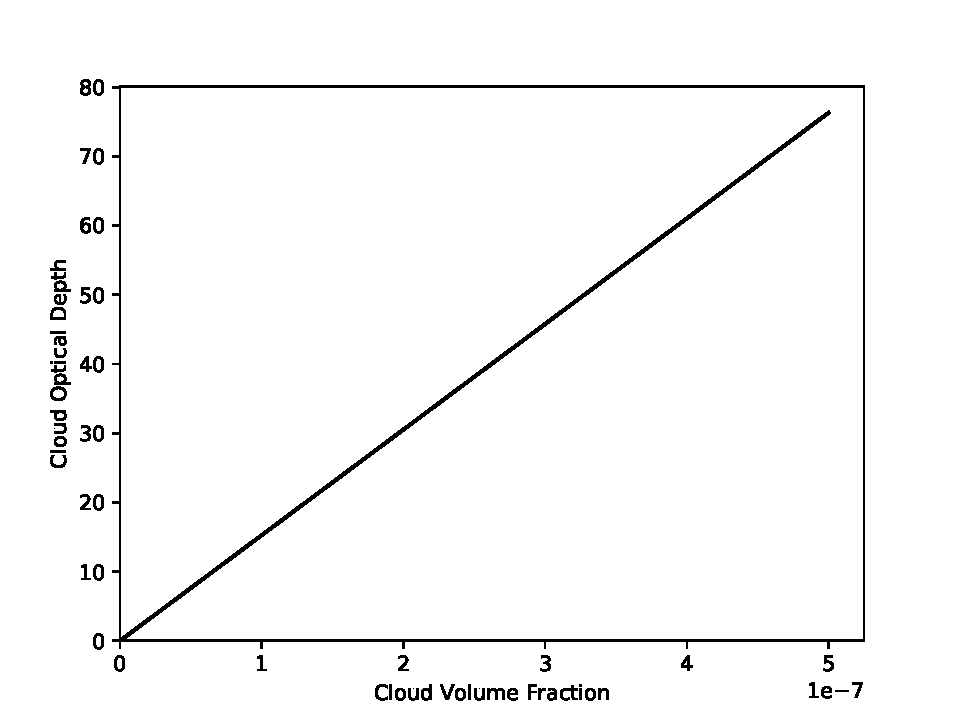
\includegraphics[width=0.7\linewidth]{COD_VS_Volf}
	\caption{$\tau_c{\scriptstyle(380 \, \text{nm})}$ versus $f_{V,c}$.}
	\label{fig:codvsvolf}
\end{figure}


The relationship between the RMF and $\tau_c{\scriptstyle(380 \, nm)}$ was investigated. 
Using AccuRT to calculate irradiances at 380 nm for different $f_{V,c}$ values yielded the theoretical relationship between RMF and $\tau_c{\scriptstyle(380 \, nm)}$ shown in Figure \ref{fig:rmfvscod380}.

\begin{figure}[H]
	\centering
	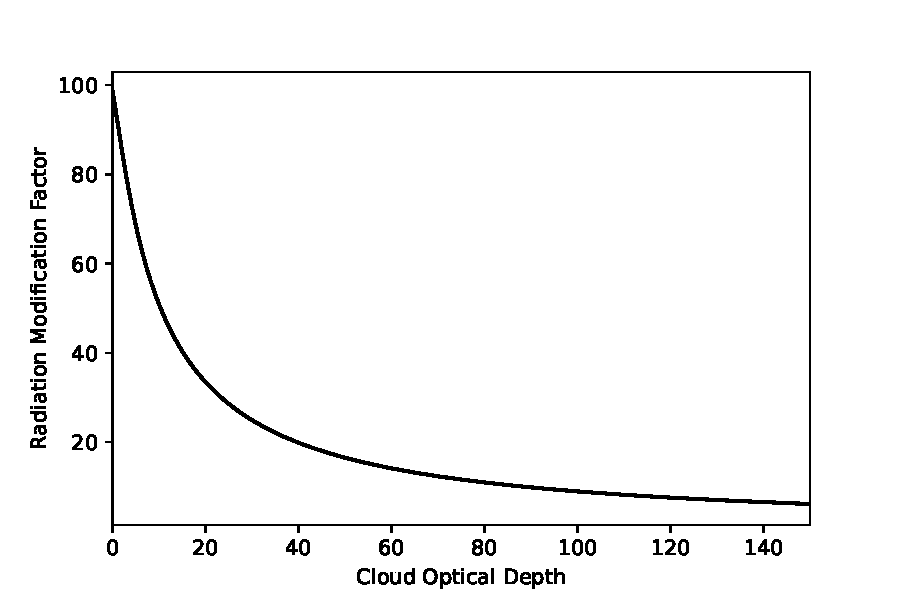
\includegraphics[width=0.7\linewidth]{RMF_vs_COD_380}
	\caption{Modeled relation between RMF and $\tau_c{\scriptstyle(380 \, nm)}$.}
	\label{fig:rmfvscod380}
\end{figure}


\section{Neural network}
\label{sec-nn}

To create a machine learning algorithm a neural network was built in Python 3 programming language with an adaptive learning rate.
Three hidden layers were set up with 100, 90, 75 neurons, respectively with hyperbolic tangent activation functions.

\textcolor{blue}{In this section the training data preparation and the two types of validation is described below.}

\subsection{Training data}

Besides taking the cosine of the solar zenith angle $\cos(\theta_0)$, to prepare the inputs ($x_i$) for the neural network training, the simulated irradiances $I_s(\lambda)$  were convolved with the absolute response functions $R_i(\lambda)$ of the corresponding NILU-UV channels.
Here $i$ denotes the channel number. 
The results of this transformation represents the voltages that would be measured in the NILU-UV channels at different irradiances.   
%Note, that there is a difference between capital $X$ which is used to denote direct inputs for the neural network, and small $x$.  
For channel 1, 3 and 5 the convolutions were the following:

\begin{equation}
	\begin{split}
		V_1 = \sum_{\lambda = 290}^{320}R_1(\lambda)I_s(\lambda) \\
		V_3 = \sum_{\lambda = 290}^{383}R_3(\lambda)I_s(\lambda) \\
		V_5 = \sum_{\lambda = 290}^{387}R_5(\lambda)I_s(\lambda) \\
	\end{split}
\end{equation}

The ratio of voltages in two channels, $\frac{V_3}{V_1}$  was used for the (TOC) prediction. 
As a reminder, our goal is to retrieve TOC and $\tau_c{\scriptstyle(380 \, nm)}$ (COD at 380 nm). 
The inputs and outputs of the neural network are gathered in {Table~\ref{tab:nn_inputs}}.

\begin{table}[H]	
	\centering
	\begin{tabular}{c|c|c|c}
		%\hline
		\textbf{input} & $\cos(\theta_0)$ &  $\frac{V_3}{V_1}$ & $V_5$ \\
		\hline
		\textbf{output} & $TOC_{scaled}$ & $f_{V,c}$ & - \\
		%\hline
	\end{tabular}
	\caption{Input and output parameters of the neural network.}
	\label{tab:nn_inputs}
\end{table}


\subsection{Holdout validation}

Once the neural network was ready for the supervised learning, the synthetic data were applied for the training.
To validate the results two procedures were done. First a 75:25 holdout, and then a K-fold validation for K=5 \textcolor{blue}{(see Section~\ref{sec-kfold})}.
For the holdout method, the mean percent error (PE), mean absolute percent error (APE) and 
\textcolor{blue}{the squared correlation coefficient ($R^2)$} were calculated using 5000 \textcolor{blue}{data-points of the neural network (NN) predictions versus the modeled results.} 
The APE and PE are defined as follows:

\begin{equation}
	\label{eq:PE}
	PE = \frac{1}{5000}\sum_{i=1}^{5000} \dfrac{NN(\underline{x}_i) - M(\underline{x}_i)}{M(\underline{x}_i)} \times 100
\end{equation}
and
\begin{equation}
	\label{eq:APE}
	APE = \frac{1}{5000} \sum_{i=1}^{5000} \dfrac{|NN(\underline{x}_i) - M(\underline{x}_i)|}{M(\underline{x}_i)} \times 100
\end{equation}
\textcolor{blue}{where $NN(\underline{x}_i)$ and $M(\underline{x}_i)$ are the results from the neural network and simulation (model)  respectively, for the $i-th$ set of parameters (or $i$-th case).}
The results predicted by the trained neural network vs. the simulated values are plotted on Figures~\ref{fig:nncodvalid} and \ref{fig:nnozonevalid}.

\begin{figure}[H]
	\centering
	\begin{minipage}{0.6\textwidth}
		\centering
		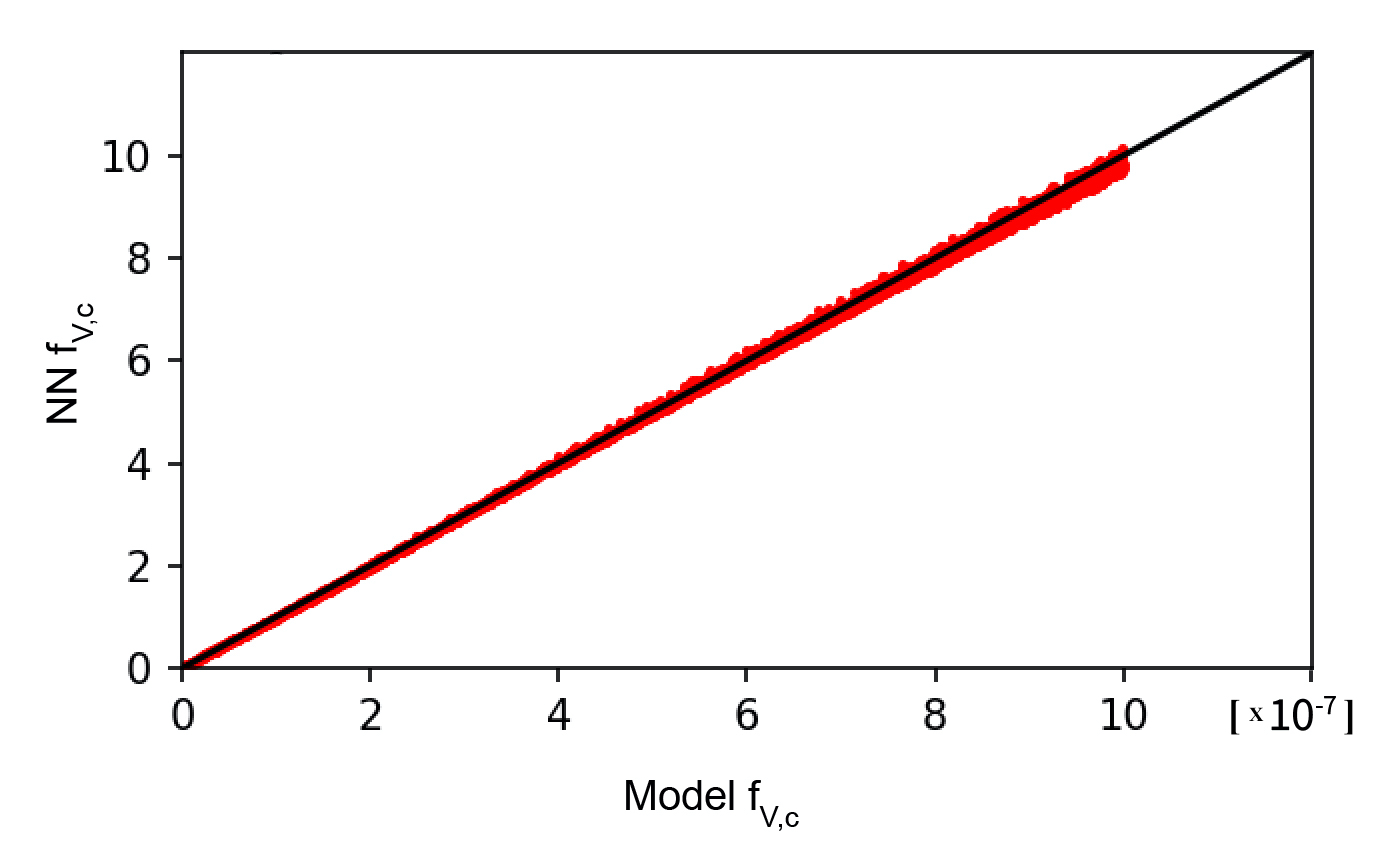
\includegraphics[width=1\linewidth]{NN_COD_val.jpg}
		\captionof{figure}{Cloud volume fraction  results by the NN vs. modeled values.}
		\label{fig:nncodvalid}
	\end{minipage}
	\begin{minipage}{0.6\textwidth}
		\centering
		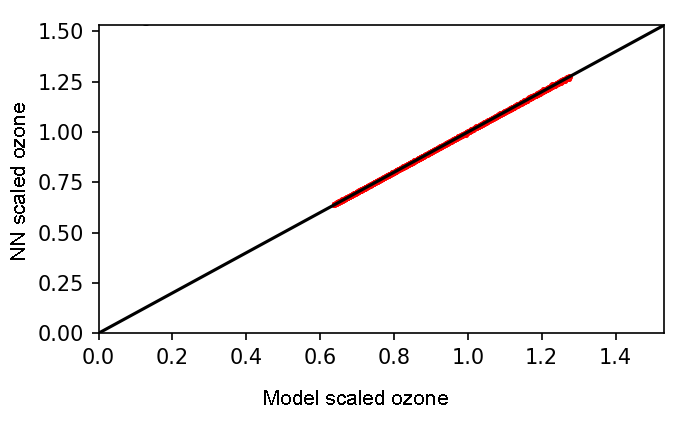
\includegraphics[width=1\linewidth]{NN_ozone_val.pdf}
		\captionof{figure}{Scaled ozone amount  results by the NN vs. modeled values.}
		\label{fig:nnozonevalid}
	\end{minipage}
\end{figure}

In Fig. \ref{fig:nnozonevalid} the $x$-axis represents the scaled ozone amount.
\textcolor{blue}{AccuRT uses scaled ozone amounts for the simulations.}
The ozone quantity is scaled to the standard US atmosphere \cite{USstandardatmosphere}, where the equivalent depth of ozone is $3.45 \times 10^{-3}$ m, which in Dobson units corresponds to 345 DU. 
The O$_3$ range in Figure~\ref{fig:nnozonevalid} from 220 DU to  440 DU is obtained by multiplying 345 DU by the factors 0.6377 and 1.2754, respectively. 
The strong correlation between the data-points is clear and the calculated statistical parameters are provided in Table~\ref{tab:nn_statistics}.

\begin{table}[H]	
	\centering
	\begin{tabular}{|c|c||c|}
		\hline
		& \textbf{O}$\bm{_3}$ & $\bm{\tau_c} {\scriptstyle(380 \, nm)}$  \\
		\Xhline{2\arrayrulewidth}
		$\bm{R^2}$	& 1 & 0.999 \\
		\hline
		$\bm{PE}$	& 0.05 \% & -0.04 \% \\
		\hline
		$\bm{APE}$	& 0.11 \%  & 1.88 \%  \\
		\hline
	\end{tabular}
	\caption{Statistical results of the neural network validation. The sample is 5000  NN predicted vs. modeled data.}
	\label{tab:nn_statistics}
\end{table}


\subsection{K-fold validation}
\label{sec-kfold}

A K-fold cross validation \cite{Hastie:2017} was also done on the training data to see how it performs on ``unseen'' data. 
A basic cross validation technique is based on partitioning a portion of the training data and utilize it to generate predictions from the neural network. 
The resulting error estimation provides insight into how the model performs on unseen data (or validation set). 
This technique is commonly referred to as the holdout method, a simple form of cross-validation.
In this case $K=5$ was adopted which is a common choice for this kind of validation method.
$K-$fold cross-validation is a technique where the dataset is divided into $K$ subsets. 
The holdout method is then repeated $K$ times, with each subset being used once as the validation set, and the remaining $K-1$ subsets being combined to form the training set. 
The error estimation is averaged over all $K$ trials to determine the overall effectiveness of our model. 
This approach ensures that each data point is included in the validation set exactly once, and in the training set $K-1$ times.  
Swapping the training and test sets further enhances the efficacy of this method. 
The statistical results  for the $K$-fold cross validation are provided in Table \ref{tab:nn_crossvalidation}.


\begin{table}[H]	
	\centering
	\begin{tabular}{|c|c||c|}
		\hline
		& \textbf{O}$\bm{_3}$  & $\bm{\tau_c} {\scriptstyle (380 \, nm)}$  \\
		\Xhline{2\arrayrulewidth}
		$\bm{R^2}$	& 0.999 & 0.999 \\
		\hline
		$\bm{PE}$	& 0.02 \% & -0.08 \% \\
		\hline
		$\bm{APE}$	& 3.27 \%  & 0.43 \%  \\
		\hline
	\end{tabular}
	\caption{Statistical results of the neural network K-fold cross validation using {$K=5$}.}
	\label{tab:nn_crossvalidation}
\end{table}

% Maybe it is not neccessary to describe the cross validation in this depth?
% Maybe it is enought just to present the k-fold validation?

\section{NILU-UV and OMI data preparation}
\label{sec-dataprep}

Once the NN was trained and validated the preparation of the NILU-UV raw data was next.  
Unfortunately some of the measurement were erroneous as the instrument logged faulty data occasionally. \textcolor{blue}{Missing datapoints, unfinished readings and appearance of random characters were the most common.}
These NILU-UV data were removed from the dataset before the following steps were taken.

The NILU-UV registers the timestamps in UTC time.
First the solar zenith angle $\theta_0$ was calculated based on the location and time. 
The other two pieces of information needed was the ratio $\frac{CH_3}{CH_1}$ and $CH_5$.
As mentioned in \cite{Sztipanov:20} section 3b, the drift factors need to be used for each channel to compensate for the instrument's Teflon diffuser's degradation. 
The nearest drift data to the measurement time was always used to take the instrument's drift into account.
The imperfect cosine response of the instrument's channels was also accounted for.

The available data after 2013 were collected from 2014 to 2019 with some days missing, mainly from year 2016.
Approximately the first third and last third of the data were lacking from 2017 and 2019, respectively.
Unfortunately because of technical difficulties NILU-UV data after 2019 was significantly gappy. 

Level 3 OMI data were acquired from NASA's Goddard Earth Sciences Data and Information Services Center (GESDISC) in hierarchical data format (release 5) for the years of interest.

\section{Results}
\label{sec-results}

\subsection{TOC results}

The retrieved TOC amounts from the NILU-UV and OMI measurements versus day of the year are plotted for the years 2014, 2015, 2018 and 2019 in Figures~\ref{fig:omil3niluo32014}, \ref{fig:omil3niluo32015}, \ref{fig:omil3niluo32018}, and \ref{fig:omil3niluo32019}. 
Plots for the years 2016 and 2017 are provided in the Appendix.\\


\begin{figure}
\begin{subfigure}[b]{0.45\textwidth}
	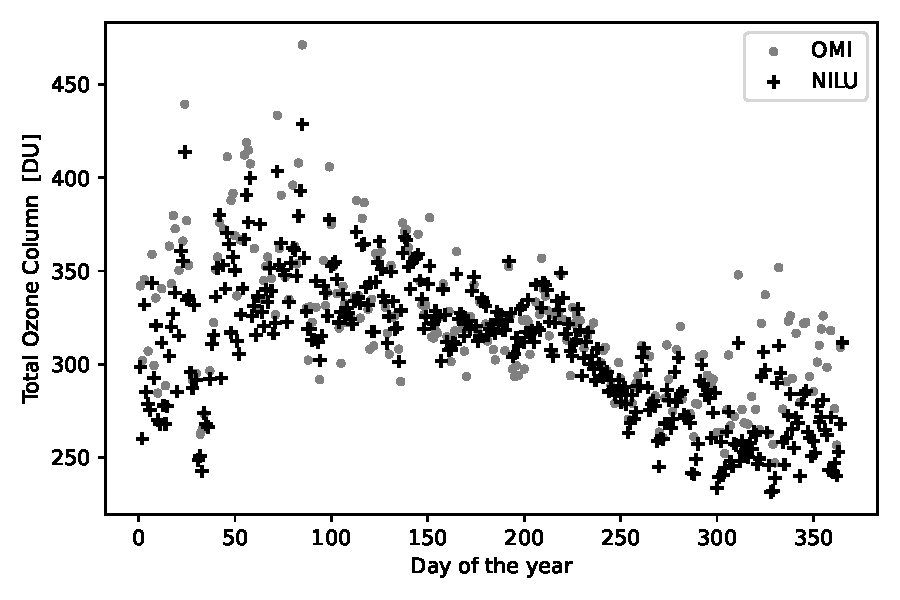
\includegraphics[width=\textwidth]{OMI_L3_NILU_O3_2014}
	\caption{}
	\label{fig:omil3niluo32014}
\end{subfigure}
\hfill
\begin{subfigure}[b]{0.45\textwidth}
	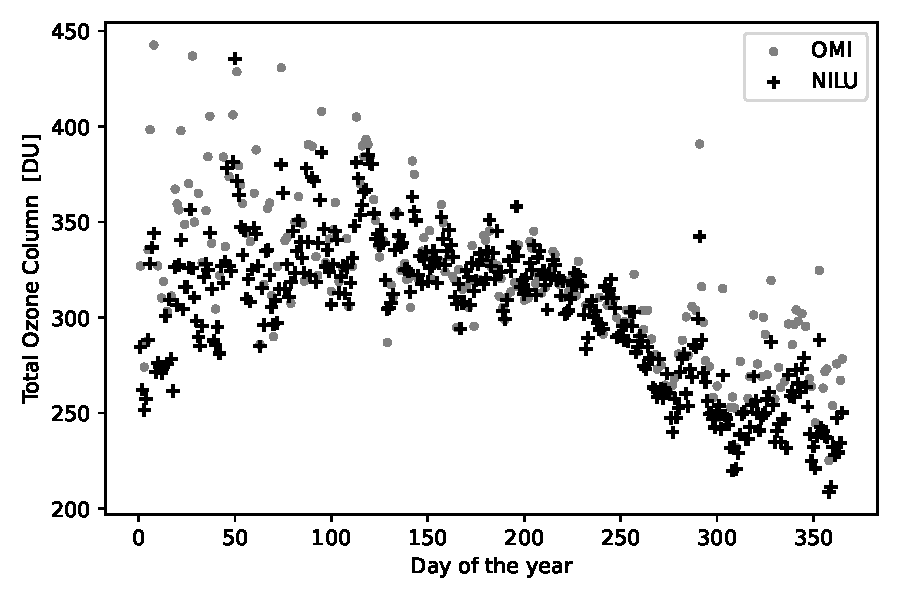
\includegraphics[width=\textwidth]{OMI_L3_NILU_O3_2015}
	\caption{}
	\label{fig:omil3niluo32015}
\end{subfigure}

\vspace{0.5cm}

\begin{subfigure}[b]{0.45\textwidth}
	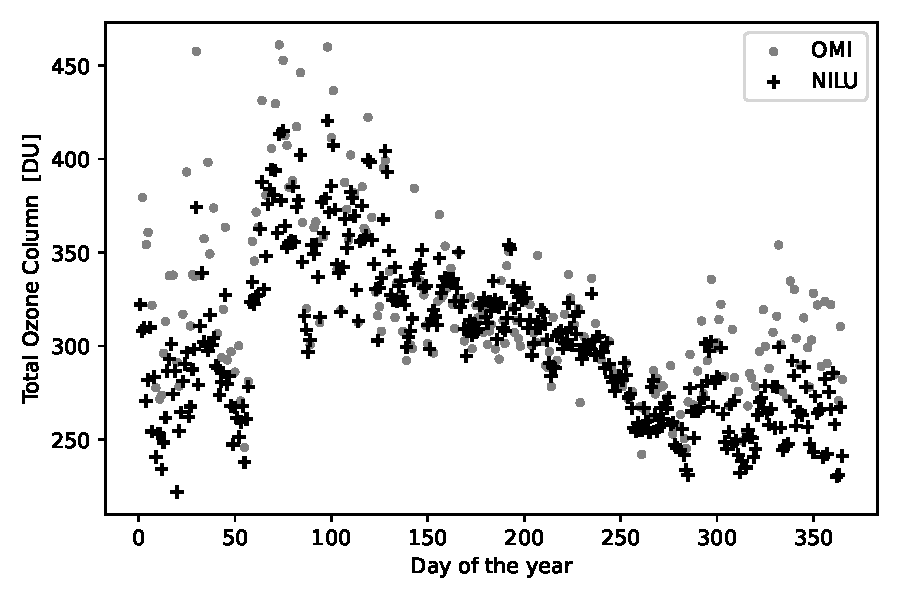
\includegraphics[width=\textwidth]{OMI_L3_NILU_O3_2018}
	\caption{}
	\label{fig:omil3niluo32018}
\end{subfigure}
\hfill
\begin{subfigure}[b]{0.45\textwidth}
	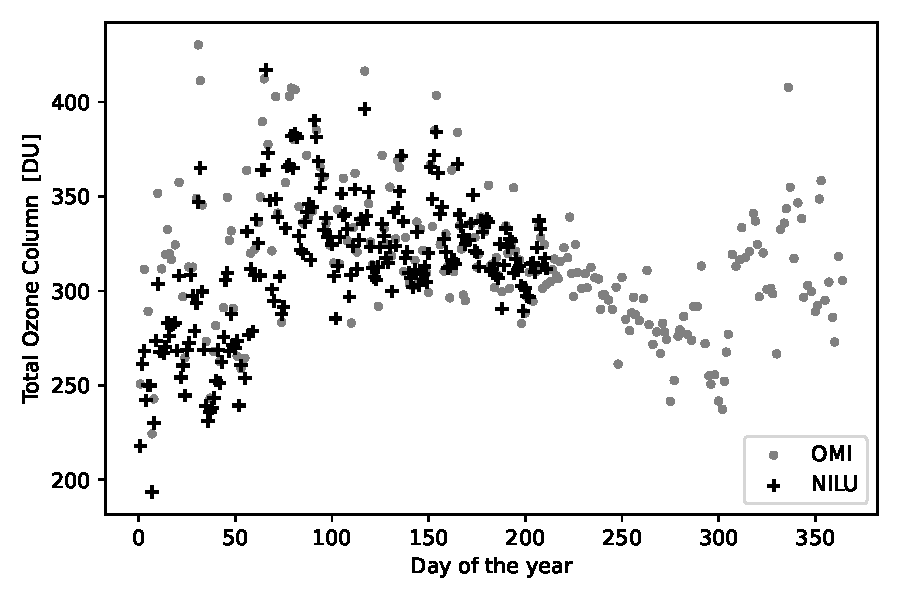
\includegraphics[width=\textwidth]{OMI_L3_NILU_O3_2019}
	\caption{}
	\label{fig:omil3niluo32019}
\end{subfigure}

\caption{TOC values from OMI (gray dots) and NILU-UV (black crosses) versus day of the year for \textbf{(a):} 2014 \textbf{(b):} 2015 \textbf{(c):} 2018 \textbf{(d):} 2019.}
\end{figure}



The plots share the same behavior, that is, the TOC values retrieved from NILU-UV tend to be lower than the corresponding OMI values. 
The same tendency was observed in ~\cite{Sztipanov:20} section 6, and as stated there, this tendency might indicate a solar zenith angle related error either in NILU-UV or OMI measurements.

For large COD values ($\tau_c{\scriptstyle(380 \, \text{nm})}$ > 100) the NILU-UV measurements showed significant TOC underestimations.
This phenomenon has already been noticed by Dahlback \cite{Dahlback:1996}, who showed that: 
(i) for clouds located between 2 and 4 km with an optical depth of $\tau_c=100$ at zero surface albedo the error in the calculated TOC is less than 2 DU compared with the TOC obtained for a cloudless sky. 
(ii) The error will increase if the surface albedo increases. In the presence of a cloud between 2 and 4 km with optical depth 
$\tau_c=100$ and a surface albedo of 0.8 the error is larger, but will not exceed 20 DU. 
(iii) At $\tau_c=50$ and surface albedo of 0.8 NILU-UV underestimates the TOC by $\sim 6\%$ \cite{Dahlback:2003}. 
In our simulations the surface albedo was adopted to be 0.14 as mentioned in Section~\ref{sec-simulations} and the $\tau_c{\scriptstyle(380 \, \text{nm})}$ occasionally exceeds 50.

Because this phenomenon occurs when the NILU-UV data analysis was done with the lookup-table method as well as with our neural network based method, it might indicate a non-linearity of the electronic components of the NILU-UV, i.e. for low irradiances (when $\theta_0$ is large or under heavy cloud cover) the instrument registers higher voltages (in channel 3) than 
it is supposed to and therefore underestimates the TOC. 
Note that this explanation is not confirmed; it is only a speculation. 
%This last paragraph might not be needed.

The annual TOC averages retrieved using the neural network, look-up table method, and OMI results, and the percent errors using OMI as a reference are listed in Table~\ref{tab:annualstats}.

\begin{table}
	\centering
	\begin{tabular}{|c|c|c|c|c|}
		\hline
		\textbf{Year} & \textbf{TOC}$_{NN}$ [DU] & \textbf{TOC}$_{OMI}$ [DU]   & \textbf{PE}$_{nn}$ [\%] & \textbf{PE}$_{lut}$ [\%]  \\
		\Xhline{2\arrayrulewidth}
		2014 & 322.70 & 322.70 & 0 & -0.23 \\
		\hline
		2015 & 318.18 & 320.15 & 0.61 & 0.70 \\
		\hline
		2016 & - & - & - & - \\
		\hline
		2017 & 305.80 & 302.67 & -0.97 & -0.18 \\
		\hline
		2018 & 320.86 & 319.80 & -0.33 & 0.21 \\
		\hline
		2019 & 323 &  319.45 & -1.1 & -0.70 \\
		\hline
	\end{tabular}
	\caption{Annual TOC results and the percent error between the annual averages.}
	\label{tab:annualstats}
\end{table}


Daily average TOC results were obtained after large COD values ($\tau_c{\scriptstyle(380 \, \text{nm})}$ > 100)  were filtered out.
This filtering led to only very small (per mille $\text{\textperthousand}$) and $\sim 0.5$ DU variance in the annual absolute and relative  differences, but it removed the outliers.
This data filtration method is an improvement compared to the suggested \cite{Hoiskar2003}  RMF < 30 limit when using the lookup-table method.
In terms of RMF,  $\tau_c{\scriptstyle(380 \, \text{nm})} = 100$ corresponds to a RMF value of 9.1.
The relationship between RMF and $\tau_c{\scriptstyle(380 \, \text{nm})}$ is plotted in Figure \ref{fig:rmfvscod380}.

%this is because there were few days like this but there is a clear limitation of the instrument. All the data ven COD > 100 were exremelly low. like ~50 DU in most cases...

The annual absolute differences ($\Delta$) using OMI as the reference, the annual relative percent errors (PE) defined by Eq.~\ref{eq:PE}, and the standard deviations ($\sigma$)  are presented in Table~\ref{tab:nnstatistics} for the TOC amounts.
\begin{table}[H]
	\centering
	\begin{tabular}{| c | c | c | c | c |}
		\hline
		\textbf{Year} & $\bm{\Delta}$ [DU] & \textbf{PE} [\%]& $\bm{\sigma}_{OMI}$ & $\bm{\sigma}_{NILU}$ \\
		\Xhline{2\arrayrulewidth}
		2014      & 13.9                    & 2.3                      & 37.4                 & 43.5                     \\
		\hline
		2015      & 12.6                       & 2                       & 38.9                  & 40.1                  \\
		\hline
		\textcolor{lightgray}{2016}      & \textcolor{lightgray}{46.5}                 &  \textcolor{lightgray}{7.4}                       & \textcolor{lightgray}{38.1}                  & \textcolor{lightgray}{31.6}                  \\
		\hline
		\textcolor{lightgray}{2017}      & \textcolor{lightgray}{16.8} & \textcolor{lightgray}{2.6}        & \textcolor{lightgray}{29.5}     & \textcolor{lightgray}{37.1}   \\
		\hline
		2018      & 16.3                      & 2.5                       & 43.0                   & 45.3                \\
		\hline
		\textcolor{lightgray}{2019}      &  \textcolor{lightgray}{16}       &  \textcolor{lightgray}{2.5}       & \textcolor{lightgray}{38}				 &  \textcolor{lightgray}{40.2}					\\
		\Xhline{2\arrayrulewidth}
		$\bm{\sum}$ & 20.4 & 3.2 & 37.5 & 39.6 \\
		\hline
	\end{tabular}
	\caption{Annual TOC statistical results for the years 2014-2019.}
	\label{tab:nnstatistics}
\end{table}

%Not sure if this table is needed at all.

As mentioned in Section~\ref{sec-dataprep}, significant amount of data from the NILU-UV measurements were missing for the years 2016, 2017, 2019, and after. 
These years are marked with light gray color in Table~\ref{tab:nnstatistics} to indicate that their higher values are not representative as an annual statistic.
Note, that these values were also included in the overall statistical results for all the years from 2014 to 2019 in the last line of Table~\ref{tab:nn_statistics}. 
The available data from these years are mainly from seasons when the daily average SZA is higher, i.e. winter. 
The higher values in Table~\ref{tab:nnstatistics} for these years supports the observation made in regards to the SZA related error in one of the instruments.

The seasonal variations and annual periodicity of the TOC in both the NILU-UV and OMI data are clearly discernible in Fig.~\ref{fig:omil3niluo3allyear}.


\begin{figure}[H]
	\centering
	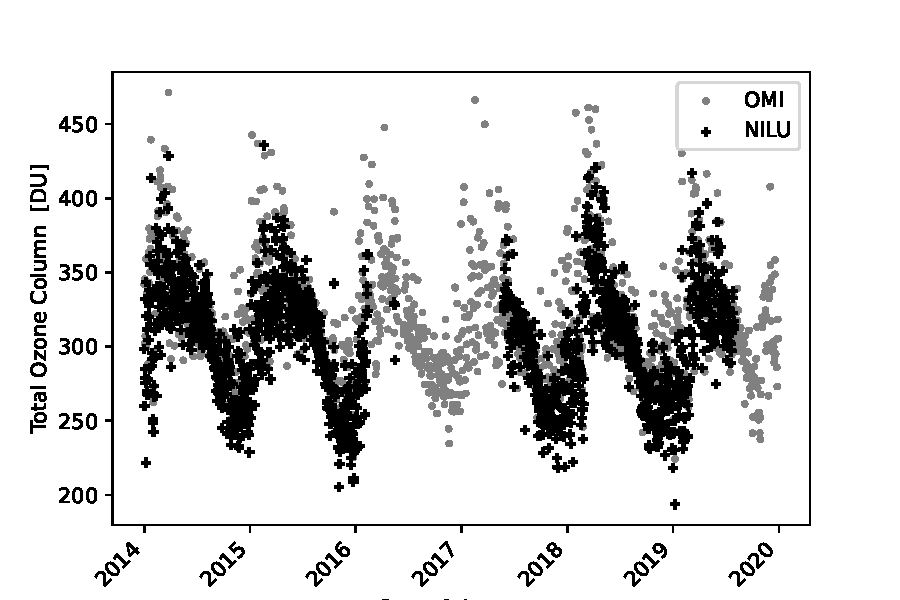
\includegraphics[width=0.75\linewidth]{OMI_L3_NILU_O3__all_year}
	\caption{The seasonal variations of TOC.}
	\label{fig:omil3niluo3allyear}
\end{figure}


The calculated annual and semi-annual variations are caused by seasonal changes in odd-oxygen production rates, temperature-dependent ozone destruction rates, and transport by the mean circulation and by eddies \cite{Perliski:1989}.

Unfortunately due to technical difficulties after 2019 the available NILU-UV data significantly dropped, but to create an up to date overview of the annual TOC amounts the missing datapoints were completed by data from OMI. The yearly TOC amount results are shown in Figure~\ref{fig:mergedtoc}.

\begin{figure}[H]
	\centering
	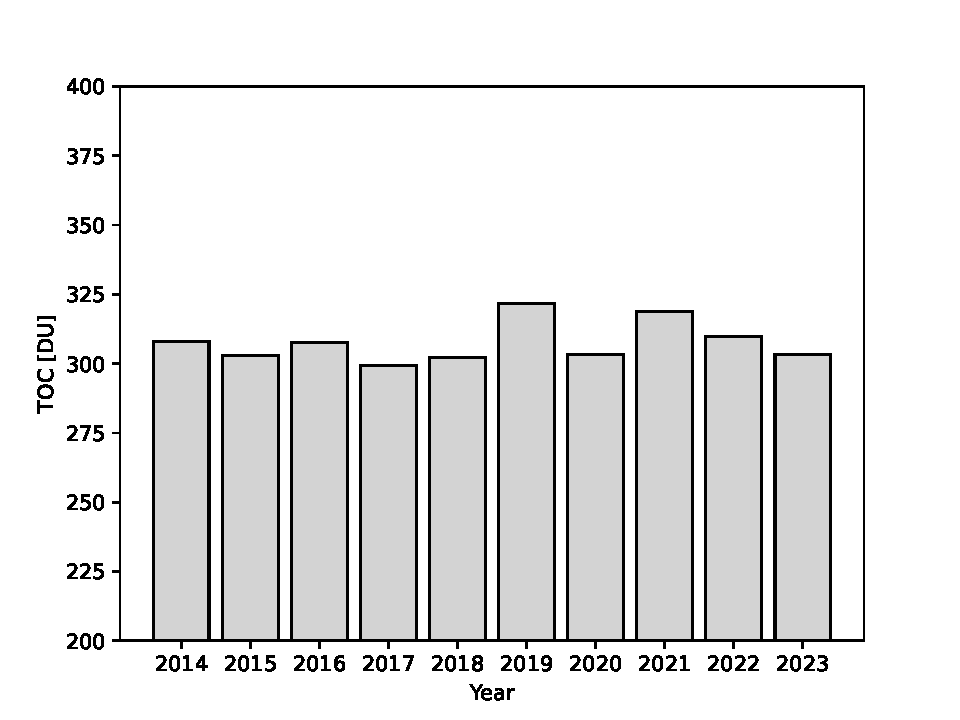
\includegraphics[width=0.7\linewidth]{mergedTOC}
	\caption{Annual TOC averages from merged data of NILU-UV and OMI between 2014-2023.}
	\label{fig:mergedtoc}
\end{figure}


\subsection{COD results}
\label{sec-codresults}

As mentioned in Section \ref{sec-simulations}, one of the outputs of the neural network is the cloud volume fraction, $f_{V,c}$.  This output was then converted to COD at 380 nm with the relationship plotted in Fig.~\ref{fig:codvsvolf}. 
The results for the years 2014, 2015, 2018, and 2019 are plotted in Figs.~\ref{fig:codvsdoy2014}--\ref{fig:codvsdoy2019}.\\



\begin{figure}
	\centering
	
	\begin{subfigure}[b]{0.45\textwidth}
		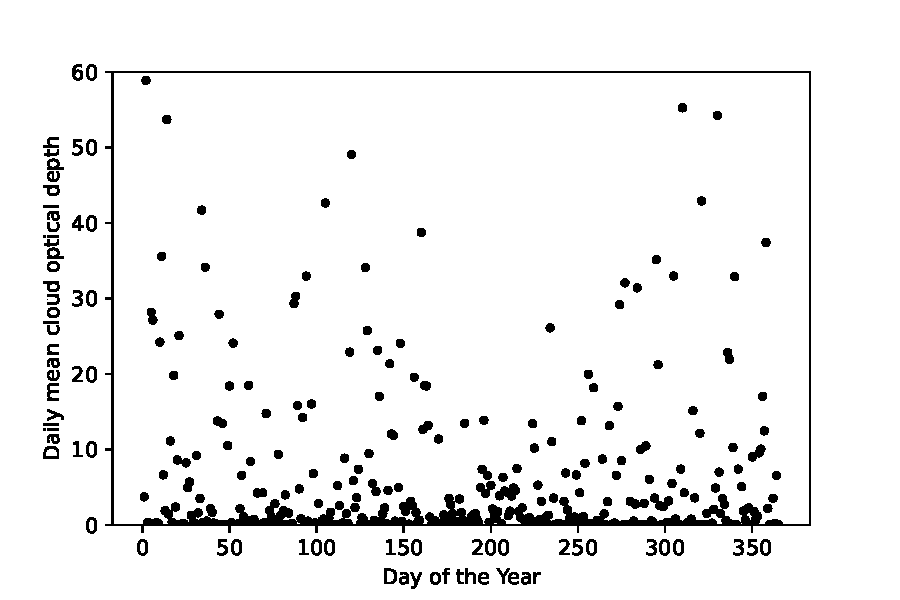
\includegraphics[width=\textwidth]{COD_vs_DOY_2014}
		\caption{}
		\label{fig:codvsdoy2014}
	\end{subfigure}
	\hfill
	\begin{subfigure}[b]{0.45\textwidth}
		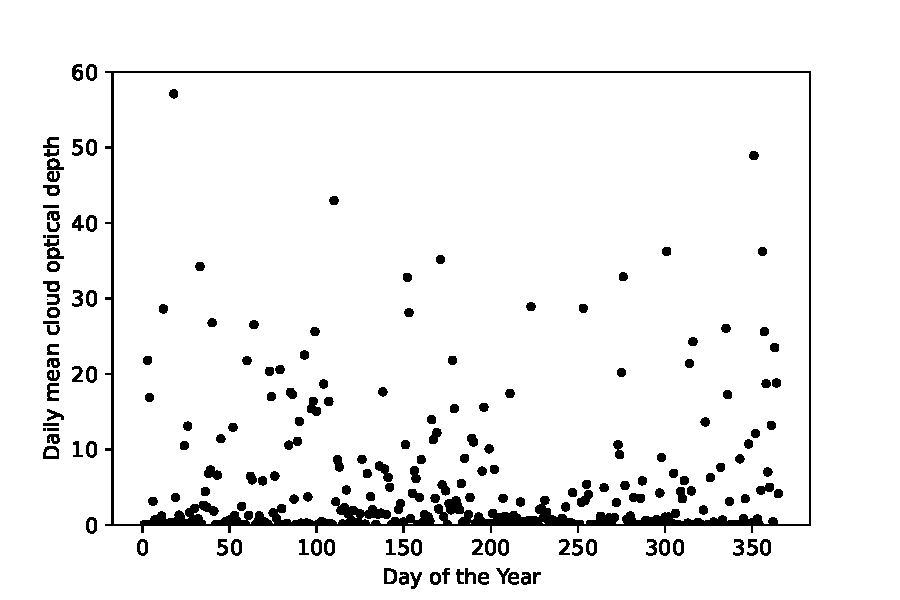
\includegraphics[width=\textwidth]{COD_vs_DOY_2015}
		\caption{}
		\label{fig:codvsdoy2015}
	\end{subfigure}
	
	\vspace{0.5cm}
	
	\begin{subfigure}[b]{0.45\textwidth}
		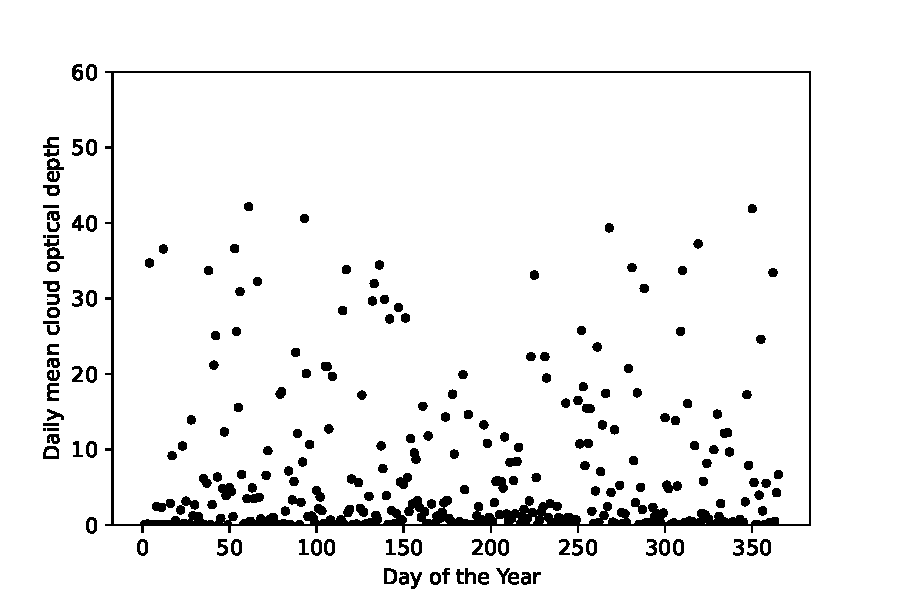
\includegraphics[width=\textwidth]{COD_vs_DOY_2018}
		\caption{}
		\label{fig:codvsdoy2018}
	\end{subfigure}
	\hfill
	\begin{subfigure}[b]{0.45\textwidth}
		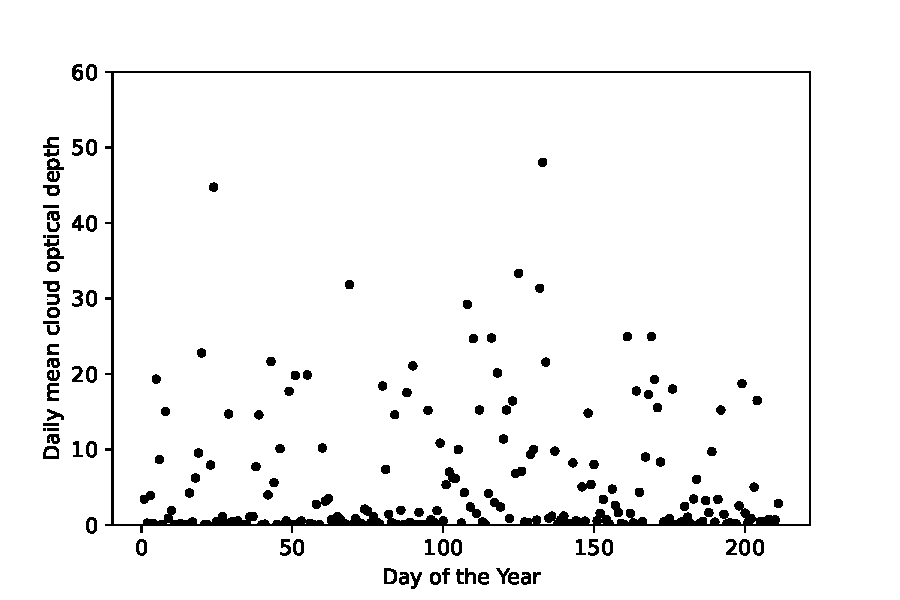
\includegraphics[width=\textwidth]{COD_vs_DOY_2019}
		\caption{}
		\label{fig:codvsdoy2019}
	\end{subfigure}
	
	\caption{Daily mean $\tau_c{\scriptstyle(380 \, \text{nm})}$ values versus day of the year for \textbf{(a):} 2014 \textbf{(b):} 2015 \textbf{(c):} 2018 \textbf{(d):} 2019.}
\end{figure}


The irradiance measurement in the 380 nm channel was chosen to derive $\tau_c{\scriptstyle(380 \, \text{nm})}$ because at this wavelength there is negligible absorption under cloud- and aerosol-free conditions, see \cite{Sztipanov:2023} Figure 7. 
The estimated error due to a presence of a heavy aerosol load (i.e. aerosol volume fraction of ${f_{V,a}} =  10^{10}$) in the atmosphere is $\tau_c(380 \, \text{nm})\; \pm \sim 3$ using a location specific aerosol model.
%this is based on fig todvf_urban+maritime. and simulations for 340nm.
The main difference between RMF and $\tau_c{\scriptstyle(380 \, \text{nm})}$ is mainly that the RMF, derived by the lookup-table method, is unreliable under broken cloud conditions and at large surface albedos \cite{Hoiskar2003}. 
Although the absorption cross section of ozone at 380 nm is close to its minimum value, and very low ($ < 10^{-24} \, \text{cm}^2$), in our neural network based method $\tau_c$ is inferred simultaneously with the ozone amount and expected to give a more reliable result. 

\section{Conclusion}
\label{sec-conclusion}

Our neural network method that retrieves TOC and COD [i.e. $\tau_c{\scriptstyle(380 \, \text{nm})}$] simultaneously from a NILU-UV instrument, showed a close agreement with the OMI results.
From the data shown in Figures~\ref{fig:omil3niluo3allyear} and \ref{fig:mergedtoc} it is clear that no alarming TOC change in the trend is noticeable. 
The lowest annual TOC amount was in 2017 with 299.4 DU. 
The highest annual average of TOC was in 2019 (321.6 DU) which might have been caused by the less than typical human activity during the COVID-19 pandemic, but because the difference being relatively not very large, and the complexity of the matter, we cannot be absolutely certain how much the declined human and industrial activity contributed to this outcome.

In contrast to the lookup-table method our neural network based method takes cloud effects into account in the TOC retrieval.
Even under heavily overcast conditions, $\tau_c{\scriptstyle(380 \, \text{nm})} > 100$, the TOC results were consistent and  showed the seasonal variation of ozone and the same patterns as the OMI measurements.
A typical choice for acceptable TOC result from the NILU-UV instrument combined with the look-up table method is when RMF $>30$ for the measurement. 
Because if the RMF is less than 30, the cloud is deemed to be too optically thick for the NILU-UV instruments to yield reliable TOC values \cite{Fan:2014b}.
The neural network method showed a significant improvement in this regard as the results are in agreement with the OMI when data with RMF $>9.1$ was set as a boundary.
%was written 7 here I need to double check, I think 9.1 is the correct number.

%\textcolor{magenta}{TOC and COD retrieval has not yet been done without the absolute calibration file of the NILU-UV instrument -- not clear ???}
% and \cite{Fan:2014b} states that: without absolute and relative calibrations, atmospheric parameters, such as the total ozone column (TOC) amount and the radiation modification factor (RMF), cannot be retrieved in a reliable manner because the sensitivity of the filters tend to drift with time.
%\textcolor{magenta}{In our method the absolute response function was used and the absolute calibration files were not. -- not clear what this statement means??}
%Utilizing the absolute response function and the relative calibration files yield a reliable result, further simplifying the retrieval. 

Assessment of the error in the COD in the presence of aerosols was provided in Section~\ref{sec-codresults}.
Beyond the previously discussed sources of error the large footprint and low time resolution of OMI (once a day) contribute to the discrepancies between results obtained from the NILU-UV and OMI instruments.
 
For the same reasons the NILU-UV is very suitable for local short- or long-term TOC, AOD, and COD monitoring. 




\section{Backmatter}

\begin{backmatter}
	
%\bmsection{Funding}
%Content in the funding section will be generated entirely from details submitted to Prism. Authors may add placeholder text in the manuscript to assess length, but any text added to this section in the manuscript will be replaced during production and will display official funder names along with any grant numbers provided. If additional details about a funder are required, they may be added to the Acknowledgments, even if this duplicates information in the funding section. See the example below in Acknowledgments. For preprint submissions, please include funder names and grant numbers in the manuscript.

%\bmsection{Acknowledgments}
%The section title should not follow the numbering scheme of the body of the paper. Additional information crediting individuals who contributed to the work being reported, clarifying who received funding from a particular source, or other information that does not fit the criteria for the funding block may also be included; for example, ``K. Flockhart thanks the National Science Foundation for help identifying collaborators for this work.'' 

\bmsection{Disclosures}
The authors declare no conflicts of interest.

\bmsection{Data availability}
The modeled synthetic data used for the neural network training and the NILU-UV raw data used in this research is available upon request from the corresponding author. All OMI data used during this study is open to the public and available from the NASA-GESDISC website \cite{NASA:gesdisc}.

\end{backmatter}

\section{Appendix}
\label{sec-appendix}

\begin{figure}[H]
	\centering
	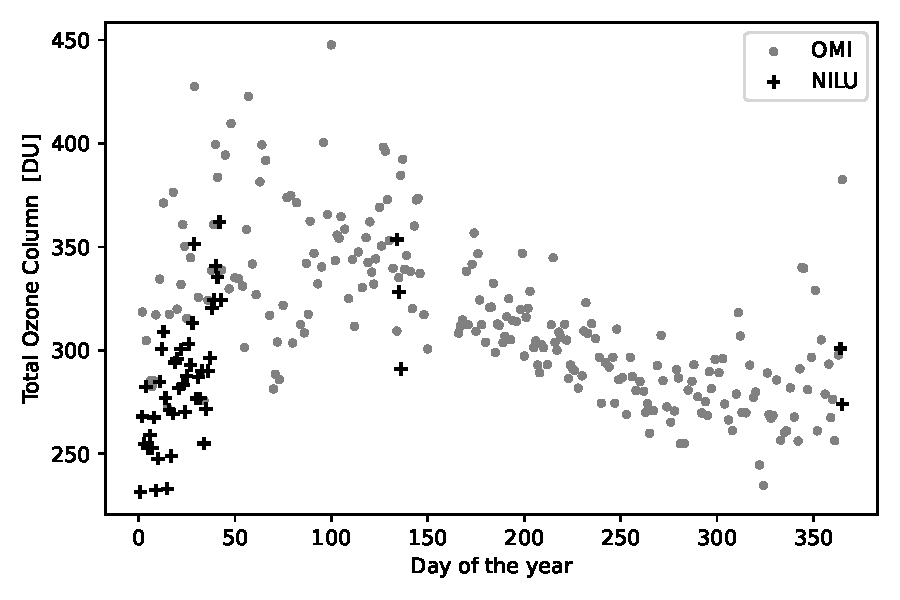
\includegraphics[width=0.7\linewidth]{OMI_L3_NILU_O3_2016}
	\caption{TOC values from OMI (gray dots) and NILU-UV (black crosses) versus day of the year for 2016.}
	\label{fig:omil3niluo32016}
\end{figure}


\begin{figure}[H]
	\centering
	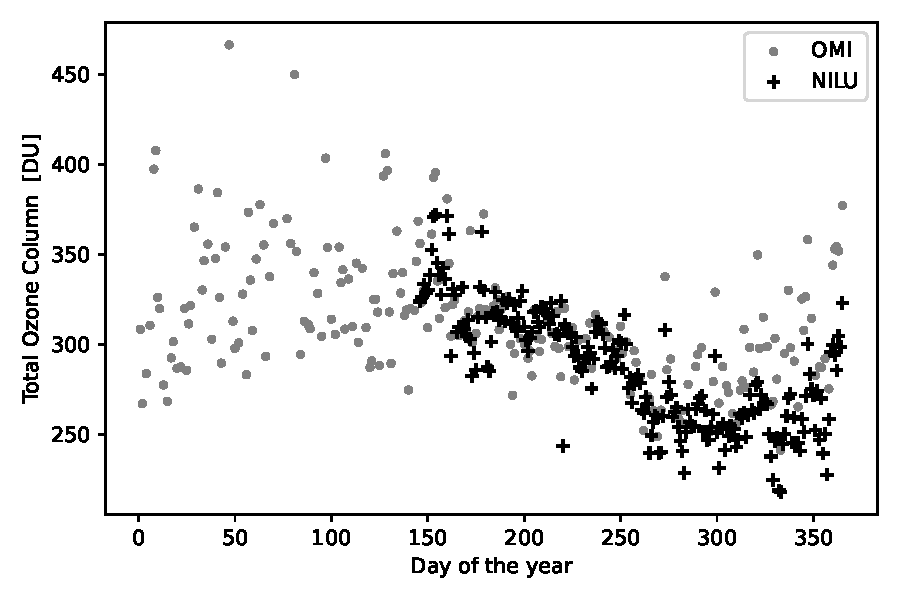
\includegraphics[width=0.7\linewidth]{OMI_L3_NILU_O3_2017}
	\caption{TOC values from OMI (gray dots) and NILU-UV (black crosses) versus day of the year for 2017.}
	\label{fig:omil3niluo32017}
\end{figure}

\begin{figure}[H]
	\centering
	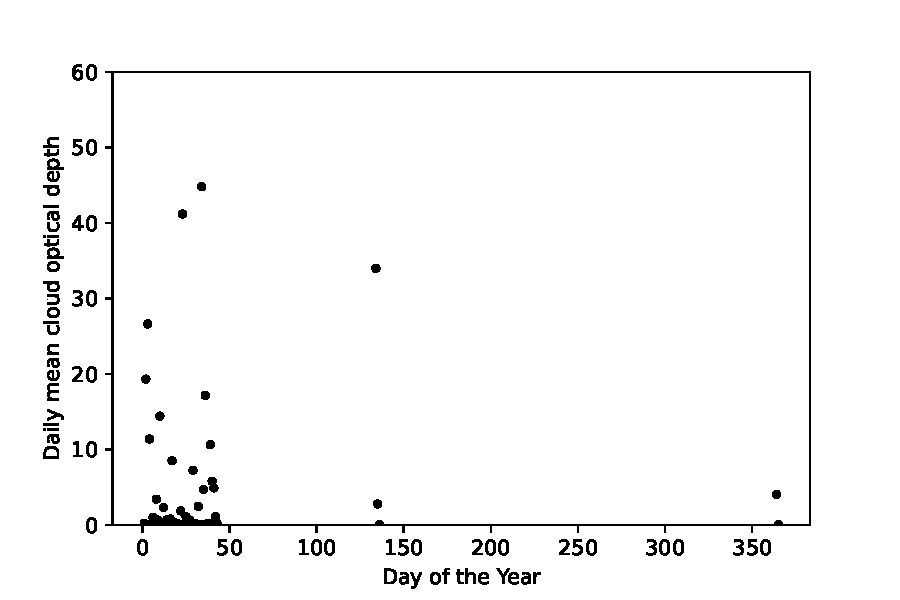
\includegraphics[width=0.7\linewidth]{COD_vs_DOY_2016}
	\caption{Daily mean $\tau_c{\scriptstyle(380 \, \text{nm})}$ values versus day of the year for 2016.}
	\label{fig:codvsdoy2016}
\end{figure}


\begin{figure}[H]
	\centering
	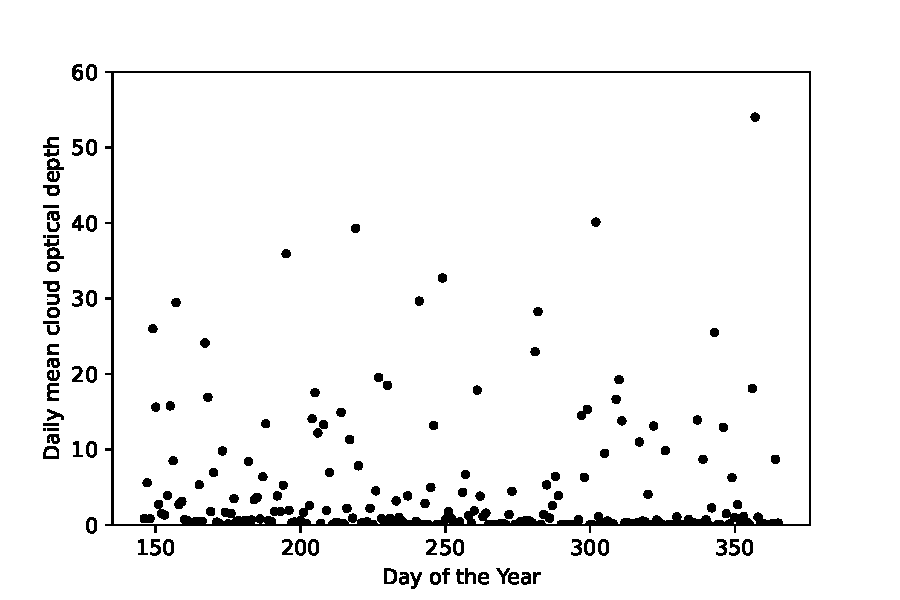
\includegraphics[width=0.7\linewidth]{COD_vs_DOY_2017}
	\caption{Daily mean $\tau_c{\scriptstyle(380 \, \text{nm})}$ values versus day of the year for 2017.}
	\label{fig:codvsdoy2017}
\end{figure}



%%%%%%%%%%%%%%%%%%%%%%% References %%%%%%%%%%%%%%%%%%%%%%%%%


\bibliography{references}



\end{document}